\documentclass{article}
\usepackage[utf8]{inputenc}

\title{Note on "Algebrization: A New Barrier in Complexity Theory"}
\author{Yu-Hsuan Huang\\asd00012334@hotmail.com \and Songfeng Wu\\sw24@illinois.edu}
\date{\today}

\usepackage{natbib}
\usepackage{graphicx}
\usepackage{amssymb}
\usepackage{amsmath}
\usepackage{algorithm}
\usepackage{fullpage}
\usepackage{times}
\usepackage{fancyhdr,graphicx,amsmath,amssymb}
\usepackage[ruled,vlined]{algorithm2e}
\include{pythonlisting}
\bibliographystyle{IEEEtran}
\setcitestyle{square}

\begin{document}

\maketitle

\section{Background}


The P versus NP problem is a main unsolved problem in complexity theory. Two main barriers have been discovered: relativization, by Baker, Gill, and Solovay\cite{baker1975relativizations}, and natural proofs, by Alexander Razborov and Steven Rudich\cite{razborov1997natural} respectively. Relativization generally states some properties of a Turing machines would still hold, when they are all given the same oracle access, i.e, the ability to instantly decide a certain language.

It has been showed that $P$ and $NP$ are equal with some oracles but they are not equal with some other oracles. And we can observe if $P \not\subseteq NP$ can be proved using relativizing proof techniques, then for any oracle $A$, $P^A \not\subseteq NP^A$. Similartly, if $P \subseteq NP$ can be proved using relativizing techniques, then the same proof can be used to show $P^A \subseteq NP^A$ for all oracle $A$. It implies that there is no relativizing proof for $P$ versus $NP$ problem. In other words, non-relativizing techniques are needed.

By analyzing some circuit lower bounds that has been proven previously, Alexander Razborov and Steven Rudich\cite{razborov1997natural} showed that if we cannot efficiently distinguish true random and psudorandom functions, then the natural proof techniques cannot be used to resolve the class $P$ and $NP$.

Some techniques have been proposed to "evade" these two barriers. To circumvent non-relativizing problem, people can use arithmetization. By evaluating a formula's 'AND', 'OR', and 'NOT' gates, it can be converted and extended into polynomials over some field while it does not have to take only $0$ and $1$ as input to its variable. In order to overcome the natural proof barrier, diagonalization was introduced. It can enumerates input strings and machines and allows us to prove some non-naturalizing problems such as $P\neq EXP$ or $\Sigma^{EXP}_2 \not\subseteq P/poly$. 

Buhrman,Fortnow,and Thierauf \cite{buhrman1998nonrelativizing} have shown that $MA_{EXP}$ is not in $P/poly$ by showing the existence of an oracle which makes the inclusion valid. Vinodchandran\cite{vinodchandran2005note} has shown that class $PP$ is not contained in class $SIZE(n$ by giving it's $n^k$ lower bounds for every $k$, which is further enhanced by Aaronson. He proved the existence of an oracle such that $PP^{A} \subseteq SIZE^A(n)$ which proved that the separation of $PP$ and $SIZE(n)$ is non-relativizing. These results indicate that some lower bounds can be shown by circumventing both barriers at the same time. 

This paper proposes a new barrier, algebraic relativization, or algebrization. It has shown that many open problems such as P versus NP, P versus RP etc., require some non-algebrizing techniques to resolve. In this paper, motivated by the truth that a Boolean formula can be considered over some fields or ring, authors extended the Boolean oracle to a low-degree extension over both fields and integers, $\mathbb{Z}$. Some concept are then clearly presented when one talks about inclusion and separation of complexity classes.

Let $C$ and $D$ be two complexity classes. $C \subseteq D$ algebrizes if $C^A \subseteq D^{\tilde{A}} $ for all oracles $A$ and all finite fields extensions of $\tilde{A}$ of $A$. $C \subseteq D$ does not algebrizes if there exist $A,\tilde{A}$ such that they make the inclusion fail, i.e. $C^A \not\subseteq D^{\tilde{A}}$. The separation is defined in a different way. $C \not\subseteq D$ algebrizes if $C^{\tilde{A}} \not\subseteq D^A$. And $C \not\subseteq D$ if there exists $A,\tilde{A}$ such that $C^{\tilde{A}} \subseteq D^A$. The paper immediately states the reason that only one class is able to access the oracle extension while the other one can only access the Boolean oracle, showing some class equivalence relation is quite difficult respect to oracle extension. 

The paper shows two main sets of concrete results, one is a set of problems that fail to relativize and can be solved by arithmetization, while all of them are shown to algebrize. They are $PSAPCE^A \subseteq IP^{\tilde{A}}$, $NEXP^A \subseteq MIP^{\tilde{A}}$, $MA^{\tilde{A}}_{EXP} \not\subset P^A/poly$, $promiseMA^{\tilde{A}} \not\subset SIZE^A(n^k)$. The other set of results that do not algebrize. They are $NP^{\tilde{A}} \subseteq P^A$, $PPACE^{\tilde{A}} \subseteq P^A$, $NP^A \not\subset P^{\tilde{A}}$, $Rp^A \not\subset P^{\tilde{A}}$, $NP^A \not\subset BPP^{\tilde{A}}$, $NP^A \not\subset BQP^{\tilde{A}}$, $NP^A \not\subset coMA^{\tilde{A}}$, $P^{NP^A}\not\subset PP^{\tilde{A}}$, $NEXP^{\tilde{A}} \subseteq P^A/poly$ and $NP^{\tilde{A}} \subseteq SIZE^A(n)$. Based on these results, the paper further demonstrates that the $P$ versus $NP$ problem will need some non-algebrizing techniques. 

\begin{figure}[!htb]
        \center{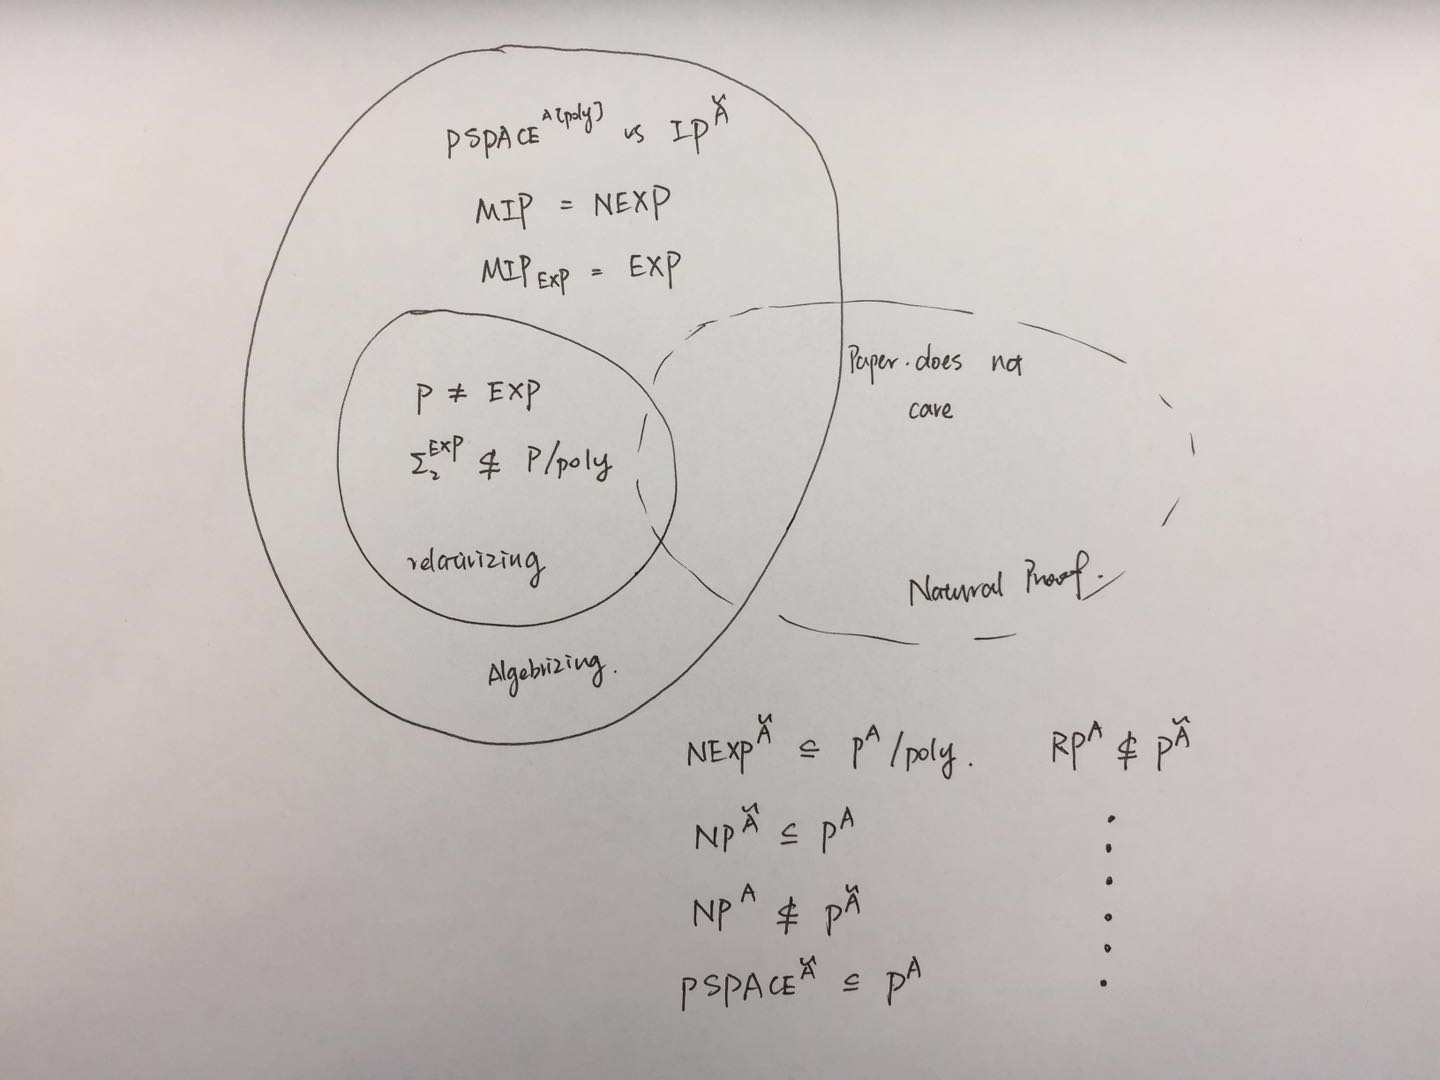
\includegraphics[width=350]
        {graph.jpeg}}
        \caption{\label{fig:my-label} Algebrization, Relativization and natrual proof}
\end{figure}



\section{Lower Bounds of Algebraic Query Complexity}

  % In standard models, an algorithm is only allowed to query an oracle $A$, a Boolean function, with some Boolean points from $\{0,1\}^n$. As oracle $A$ is extended to low-degree $\tilde{A}$ over fields $\mathbb{F}^n$, proving some lower bounds respect to the query complexity can be helpful with showing oracle separation later.
  With an oracle $A:\{0,1\}^n\rightarrow\{0,1\}$ extended to a low-degree polynomial $\tilde{A}$, the paper introduce the notion of algebraic query complexity. By allowing queries on non-Boolean inputs, it is natural to ask whether our oracle machines are granted with more power? The answer is no, in the sense that several lower bounds are given, and from that, the paper constructs adversary polynomials to prove seperations in algebrized worlds.

  %We first do some set up. For $N=2^n$, let $f:\{0,1\}^N\rightarrow\{0,1\}$ be a distinguisher function taking oracle $A: \{0,1\}^n \rightarrow \{0,1\}$ as input. Let $\tilde{A}$ be an oracle extension of $A$ over field $\mathbb{F}$. Note that the field can be infinite if it is not specified to be finite. We now introduce the notion of delta basis, for $z\in\{0,1\}$, define $\delta_z(x) := \prod\limits_{i:z_i=1}x_i \prod\limits_{i:z_i=0}(1-x_i)$ as a multilinear polynomials that outputs $1$ at $z$ and $0$ at elsewhere in $\{0,1\}^n$. Collection of delta functions among Boolean $z$'s $\{\delta_z:z\in\{0,1\}^n\}$ forms a basis of multilinear polynomial space. Let $m$ be an arbitrary multilinear polynomial, it could be uniquely represented as linear combination of the delta basis $\delta_z$'s as $m(x) = \sum\limits_{z\in \{0,1\}^n}m_z\delta_z(x)$ where $m_z\in\mathbb{F}$.
  We first do some set up. For $N=2^n$, let $f:\{0,1\}^N\rightarrow\{0,1\}$ be a distinguisher function taking oracle $A: \{0,1\}^n \rightarrow \{0,1\}$ as input. Let $\tilde{A}$ be an oracle extension of $A$ over field $\mathbb{F}$. We now introduce the notion of delta basis, for $z\in\{0,1\}$, define $\delta_z(x) := \prod\limits_{i:z_i=1}x_i \prod\limits_{i:z_i=0}(1-x_i)$ as a multilinear polynomials that outputs $1$ at $z$ and $0$ at elsewhere in $\{0,1\}^n$. Collection of delta functions among Boolean $z$'s $\{\delta_z:z\in\{0,1\}^n\}$ forms a basis of multilinear polynomial space. Let $m$ be an arbitrary multilinear polynomial, it could be uniquely represented as linear combination of the delta basis $\delta_z$'s as $m(x) = \sum\limits_{z\in \{0,1\}^n}m_z\delta_z(x)$ where $m_z\in\mathbb{F}$.
  
  In deterministic models, given a Boolean function $f$, its query complexity $D(f)$ is defined as the minimum number of queries required to compute $f$. In algebraic query complexity model, it's complexity is defined over fields as the following. Consider a collection $\mathcal{M}$ of deterministic algorithms $M$ such that $M^{\tilde{A}}$ outputs $f(A)$ for every oracle $A$ and every finite field extension $\tilde{A}$ with mdeg{$\tilde{A}$} $\le c$, where c is a positive integer. The deterministic algebraic query complexity $\tilde{D}_{\mathbb{F},c}(f)$ of $f$ is defined to be $\min\limits_{M \in \mathcal{M}} \max\limits_{A,\tilde{A}: mdeg(\tilde{A}) \le c} T_M(\tilde{A})$ , where $T_M(\tilde{A})$ is the number of queries to $\tilde{A}$ made by $M^{\tilde{A}}$. Note that $\tilde{R}_{\mathbb{F},c}(f)$ is defined in the same manner respect to the randomized model.
  
  Let $y_1,\dots,y_t $ be points in $\mathbb{F}$. We can observe that there exists a multilinear polynomial $m: \mathbb{F}^n \rightarrow \mathbb{F} $ such that $m(y_i)=0 $ for all $i \in [t]$ and $m(z) = 1$ for at least $2^n-t$ Boolean points. Further, for at least  $2^n-t$ Boolean points $w \in \{0,1\}^n$, there exists a multiquadratic extension polynomial $p$ such that $p(y_i)=0$ for all $i \in [t]$, $p(w) = 1$ and $p(z) = 0$ for all Boolean $z \neq w$. Let $\mathcal{Y} \subseteq \mathbb{F}^n $. We call a Boolean point $w$ good if for every $\mathbb{F}\in\mathcal{F}$, there exists a multiquadratic polynomial $u_{\mathbb{F},w}$ such that $(1)$ $u_{\mathbb{F},w}(y)=0$ for all $y\in\mathcal{Y}_{\mathbb{F}}$, $(2)$ $u_{\mathbb{F},w}(w)=1$ and $(3)$ $u_{\mathbb{F},w}(z)=0$ for all Boolean points $z\neq w$.
 
 \subsection{Deterministic Results}
  
  As what we have learnt in the lecture, define $OR$ be a distinguisher that on input oracle $A_n:\{0,1\}^n\rightarrow\{0,1\}$, decides whether there exists an length$-n$ $x \in \{0,1\}^n$ such that $A_n(x) = 1$. Consider a deterministic algorithm with access to extension oracles $\tilde{A}_{n,\mathbb{F}}$ which query a set of points $\mathcal{Y} \subseteq \mathbb{F}^n$ with $|\mathcal{Y}| < 2^n$. There is a multiquadratic extension $\tilde{A}$ of $A$ that ellimniate $\mathcal{Y}$, i.e. $\forall y\in\mathcal{Y}: \tilde{A}(y)=0$ with another Boolean point $w$ that $\tilde{A}(w)=1$. Therefore, such algorithm cannot distinguish between $\tilde{A}$ and trivial oracle extension, $\forall x\in\mathbb{F}^n:x\mapsto 0$. And we are left with an exponential lower bound $\tilde{D}_{\mathbb{F},2}(OR)=2^n$.
  
  
  \subsection{Probablistic Results}
  
  Then the paper shows some results on probabilistic lower bounds respect to randomized algorithms. In order to introduce the lower bound $\tilde{R}_{\mathbb{F},2}$, we  first need to consider the following. For all $w\in\{0,1\}^n$, let $D_w$ be the uniform distribution over multiquadratic polynomial $p: \mathbb{F}^n \rightarrow \mathbb{F}$ (filed $\mathbb{F}$ needs to be finite here) such that $p(w)= 1$ and $p(z)=0$ for all other Boolean points $z$. Think of that the algorithm chooses a $w$ uniformly at random and a $p$ according to the $D_w$. The paper shows that the probability of a deterministic algorithm $DA$ will have queried the chosen $w$ is at most $\frac{t}{2^N}$ where $t$ is the number of queries that it has made to polynomial $t$. It can be seen in the following way. Let $\{y_i | y_i\in \mathbb{F}^n\}_{i\in[t]}$ be a set of points that queried by the algorithm. Let $G_t$ be the set of good points immediately after $t^{th}$ step, and $u$ be the  multiquadratic polynomial in the definition of good point. Let $B_t = \{0,1\}^n / G_t $ denotes the set of bad points against the good points. Since non of $y_i$'s are good, then $|G_t| \ge 2^n - t$ and $B_t \le t$. It is clear that $B_t \subseteq B_{t+1}$ for all t. For all good points $z$, fix a $u_z$ for it(since there might be a couple of such $u$ that let $z$ be a good point). By conditional probability, We know 
 
 \begin{center}
     $Pr[\text{After t steps, DA will have queried the chosen point w}] = $ $ \sum\limits_{i=0}\limits^{t-1} Pr[ \text{w is queried in the step } i+1 | \text{w was not queried in the first i steps}] $ $ Pr[\text{w was not queried in the first i steps}]$     
 \end{center} 
 
 It is clear that $Pr[\text{w was not queried in the first i steps}] = \frac{2^n - |B_i|}{2^n}$. Note that after $t$ steps, there are $|G_t| = 2^n - |B_t|$ points have not been queried. Observe that each point is equally likely to be $w$. Note that there are at most $|G_t| - |G_{t+1}| =  (2^n - |B_t|) - (2^n-|B_{t+1}|) = |B_{t+1}| - |B_t|$ number of 'new' Boolean points that can be queried in step $t+1$. Notice that if the point $y_{i+1}$ queried by the $DA$ in step $i+1$ is Boolean, then $y_{i+1} \in B_{t+1}$. And we know $w$ is a Boolean as we mentioned at the very beginning. Thus
 
 \begin{center}
     $Pr[ \text{w is queried in the step } i+1 | \text{w was not queried in the first i steps}] = $ $\frac{|G_t|-|G_{t+1}|}{G_t} = \frac{|B_{t+1}| - |B_t|}{2^n - |B_t|}$ 
 \end{center}
 
 
  Hence,
  
  \begin{center}
       $Pr[\text{After t steps, DA will have queried the chosen point w}] = $ $ \sum\limits_{i=0}\limits^{t-1} (\frac{2^n - |B_i|}{2^n})(\frac{|B_{t+1}| - |B_t|}{2^n - |B_t|}) $ = $\sum\limits_{i=0}\limits^{t-1} (\frac{|B_{t+1}| - |B_t|}{2^n}) \le \frac{t}{2^n}$
  \end{center}
  
  Based on this intermediate result , the paper emphasizes that the randomized query algorithms cannot do better than the deterministic versions at evaluating the $OR$ problem. We use the same definition of the $OR$ problem. Similar to what was proved for the deterministic case but this time letting the deterministic algorithm randomly chooses a marked Boolean point $w$. Then by the above proof, there is a multiquadratic extension $\tilde{A}$ of $A$ that eliminates all Boolean points other than $w$, i.e. $\forall z \in \{0,1\}^n, z \neq w : \tilde{A}(z)=0$ and $\tilde{A}(w)=1$. By the proof, after making $t$ queries to $\tilde{A}$, the probability of $w$ will have been queried is at most $\frac{t}{2^n}$. Notice that when $t$ is greater than $2^n$, then the probability becomes $1$, which is trivial. It follows that the number of queries is at most $2^n$, i.e. $\tilde{R}_{\mathbb{F},2}(OR) = \Omega(2^n)$.
  

  \subsection{Lower Bound Respect to Communication Complexity}
  
  Further, the paper shows how the algebraic query algorithms can be efficiently simulated by Boolean communication protocols, which give people more power on proving some hard lower bound of algebraic query complexity. Let $A: \{0,1\}^n \leftrightarrow \{0,1\}$ be a Boolean function and $\tilde{A}: \mathbb{F}^n_q \rightarrow \mathbb{F}_q$ be the unique multilinear extension of $A$ over a finite field. Suppose $f(A)$ can be evaluated by querying $\tilde{A}$ $T$ times, where $f$ is the Boolean predicate of $A$. Let Alice and Bod hold the truth table of subfunctions $A_0$ and $A_1$ respectively where $A_0$ and $A_1$ are two functions obtained by restricting the first bit to $0$ or $1$. Let $M$ be an algorithm evaluating $f$ using $T$ queries to $\tilde{A}$. For any query poin $y$ to $\tilde{A}$, we can write $\tilde{A} = \sum\limits_{z\in\{0,1\}^n} \delta_z(y)A(z)$. It follows that Alice and Bob can do the partial sum check with functions $A_0$ or $A_1$ in hand. Briefly, Alice computes $\tilde{A_0}(y_i) := \sum\limits_{z\in\{0,1\}^{n-1}} \delta_{0z}(y_i)A(0z) $ and sends $(y_i,\tilde{A_0}(y_i))$ to Bob. Then Bob computes $\tilde{A_1}(y_i) := \sum\limits_{z\in\{0,1\}^{n-1}} \delta_{1z}(y_i)A(1z) $ and from which he will have $\tilde{A}(y_{i}) = \tilde{A_0}(y_{i}) + \tilde{A_1}(y_{i})$ to obtain the next query point $y_{i+1}$ and sends $(y_{i+1},\tilde{A_1}(y_{i+1}))$ to Alice. Then a new round starts. This sum check process will be repeated for $T$ rounds. It is clear that the communication protocol simulates the algotithem $M$ step by step. Note the total communication cost is $TO(nlog|\mathbb{F}|) = O(Tnlog|\mathbb{F}|)$. 
  
  Define the Disjointness problem as the following. Let $x=x_1,\dots,x_N$ and $y=y_1,\dots,y_N$ be two Boolean strings. The problem is to decide whether there exists an index $i$ s.t. $x_i = y_i = 1$. The problem can be reformed by using the above definition as given a Boolean function $A: \{0,1\}^n \rightarrow \{0,1\}$, decide whether there exists an $x\in\{0,1\}^{n-1}$ s.t. $A(0x) = A(1x) = 1$. If we think of an randomized algorithm which queries the multilinear extension $\tilde{A}$ of $A$ above, then it can be seen that $\tilde{R}_{\mathbb{F},1}(Disjointness) = \Omega(\frac{2^n}{nlog|\mathbb{F}|})$ by setting up a contradiction to the result done by Razborov\cite{razborov1990distributional} and Kalyasundaram and Schnitger\cite{kalyanasundaram1992probabilistic}.

\section{Algebrizing Complexity Classes}
  
\subsection{Algebrizing IP v.s. PSPACE}

The notion of algebrization is defined combining the concept of relativization and arithmetization, Let's take a look at prior proof for $IP=PSPACE$ by Shamir \cite{shamir1990ip}. We (interactively) prove/disprove a quantified boolean formula $\phi\in TQBF$. Define $f_i(x_i)\equiv Qx_{i+1}...Qx_{n}\phi(r_1,...,r_{i-1},x_i,...,x_n)\forall x_i\in\{0,1\}$ and $f_i(x_i) = f_i(0)(1-x_i)+f_i(1)x_i$, {\bf Algorithm 1} sketch the proof given by Shamir.

\begin{algorithm}[H]
\SetAlgoLined
%\KwResult{Solving TQBF}
 %initialization\;
 %\For{}{} \While{}{}
 Prover sends $\tilde{f_0}=1$\;
 
 \For{i=1..n}{
   Prover sends $\tilde{f_i}$, claiming it is $f_i$\;
   \eIf{$\tilde{f_i}\equiv f_i$ on boolean input}{ 
        \eIf{the claimed value of $\tilde{f}_i$ matches $\tilde{f}_{i-1}$}{
            Verifer sends back a random $r_i\in\mathbb{F}$\;
        }{reject\;}
   }{reject\;}
 }
 
 Verifier checks \eIf{$\tilde{f}_n=f_n=f(r_1,...,r_n)$}{accept\;}{reject\;}
 \caption{IP protocol solving TQBF}
\end{algorithm}

Note that in  the last step, we need to evaluate $f_n=f(r_1,...,r_n)$, if we now allow our quantified formula with access to some oracle gate $A:\{0,1\}^*\rightarrow\{0,1\}$ with un-bounded fan-in, evaluation of $A(r_{i_1},...,r_{i_k})$ would be done by giving the verifier with oracle access to its oracle extension $\tilde{A}$, then we would have exactly the same algorithm works (in the algebrized world), thus $PSPACE^{A}\subseteq IP^{\tilde{A}}.$ By introducing oracle access to an arithmetized Boolean formula, algebrization would naturally occur.

\subsection{Algebrizing Barrier of P v.s. NP}
P vs NP is one of the well known problem, relativization barrier has alrealdy been discovered, the paper took one further step showing that it is as well non-algebrizing. Let's recall the proof given by Baker, Gill and Solovay\cite{baker1975relativizations}. It suffices to show existence of languages $A,B$ that $P^A=NP^A$ and $P^B\neq NP^B$. For the former, we choose $A$ so hard, that difference of $P, NP$ becomes small. In particular, choose $A=TQBF$ that determined whether an input quantified Boolean formula is true. Then we will have
$$
P^{TQBF}=PSPACE=NP^{TQBF}.
$$
For the latter, choose $OR^B=\{1^n:\exists x\in\{0,1\}^n,x\in B\}$ to seperate $P^B, NP^B$. Diagonalization is used to construct such $B$. Roughly speaking, consider an enumeration of poly-time oracle machine, $\{M_i\}.$ Note that we do not need to provide which oracle given to $M_i.$ Beacuse the family of all possible oracles are too large, number of queries will only be a "sparse" subset of $B$, that gives us some freedom constructing $B$ to differ $OR^B$ from $L(M_i^B)$. We incrementally construct the language $B$ with a process that decides $B_0\subseteq B_1\subseteq B_2\subseteq\cdots\subseteq B$. Specifically, if $M_i^B$ accept $1^{n_i}$, we choose $B_{i+1}$ containing no length$-n_i$ strings. Otherwise, if $M_i^B$ reject $1^{n_i}$, we choose a not-yet-queried point $x\in\{0,1\}^{n_i}$, and set it in $B_{i+1}$. Thus, we have
$$
OR^B\in P^B-NP^B.
$$

\subsubsection{Proof of $P\neq NP$ Non-algebrizing}
In this part, we essentially want to show that $NP^{\widetilde{TQBF}}\subseteq P^{TQBF}$. By Babai, Fortnow and Lund's result\cite{babai1991non}, the multi-linear extension of a $PSPACE$ oracle could be computed with an $IP$ protocol, and thus can be simulated by a polynomial space machine. Therefore we have,
$$
NP^{\widetilde{TQBF}}\subseteq PSPACE=P^{TQBF}.
$$

\subsubsection{Proof of $P=NP$ Non-algebrizing}
Similar technique is used when proving this part, we are picking $B=\bigcup_i B_i$ such that $OR^B$ would separate $NP^{B}, P^{\tilde{B}}$. Since obviously $OR^B\in NP^B$, it suffices to show $OR^B\not\in P^{\tilde{B}}$ This follows from the circuit lower bound at {\bf section 2.1}
$$
\tilde{D}_{\mathbb{F},2}(OR)=2^n.
$$
In another word, there's a setting of oracles, $\{S_i=B_i-B_{i-1}\}$ that each $S_i:\mathbb{F}^{n_i}\rightarrow \mathbb{F}$ requires $2^{n_i}$ queries in $\mathbb{F}^{n_i}$ to determine the value of $OR(S_i)$, hence
$$
OR^B\not\in P^\tilde{B}.
$$

\section{Algebrization over Integer}
Algebrization could also be established on $\mathbb{Z}$. The corresponding oracle extension $\hat{A_n}$ could be defined as the constant degree integer polynomial that agrees with $A_n$ on boolean input. Furthermore, we require such oracle will only give outputs that are polynomially bounded, i.e. $\forall x\in\mathbb{Z}^n$, $size(\hat{A}_n(x))\leq poly(n+size(x))$. Similarly, the algebraic query complexty \hat{D_{s,t}} is defined as the minimum worst case number of the oracle queries $\hat{A_n}$ needed wehn computing distinguisher's output $f(A)$, except that we require our input x to have bounded size $size(x)\leq s$.

\subsection{Algebraic Fact}
To further extend the results, we now introduce some well known fact. Namely, we will use Chinese remainder theorem to stack co-prime results together and Hensel lifting to address prime power case. Here, we restrict our discussion respect to integers.

\subsubsection{Chinese Remainder Theorem}
Given $m,n$ be co-prime positive integers, we'll have the ring isomorphism $\mathbb{Z}_{mn}\cong \mathbb{Z}_m\times \mathbb{Z}_n$. Consider the ring homomorphism $\psi:\mathbb{Z}\rightarrow \mathbb{Z_m}\times\mathbb{Z_n}$ defined by $l\mapsto (l\mod m, l\mod n)$, because $m,n$ are co-prime, we have $\ker\phi=mn\mathbb{Z}$ thus
$$
\mathbb{Z}_{mn}=\mathbb{Z}/\ker\phi\cong \phi(\mathbb{Z})=\mathbb{Z}_m\times\mathbb{Z}_n.
$$
\subsubsection{Hensel Lifting}
Given a matrix $A\in\mathbb{Z}^{n\times n}$ invertible under $\mathbb{Z}_q$ for prime $q$, the linear equation $Ax=b$, for arbitrary $b\in\mathbb{Z}^n$, will have solution mod arbitrary prime $q$-power $\mathbb{Z}_{q^e}$. Suppose $x'=x\mod q^{e-1}, b'=b\mod q^{e-1}, y\in\mathbb{Z}^n$, then we will have
$$
b=Ax=A(x'+q^e\cdot y).
$$
Restrict this equation to $\mathbb{Z}_{q^{e-1}}$, we will have $q^e\cdot A y=0\mod q^{e-1}$. Therefore, by constructing solution of $y$ to $Ay=0\mod q^{e-1}$ recursively, we will have $x=x'+q^e \cdot y$ do exists.


\subsection{Multi-linear Lower Bound}
We first strip down some field constraint in previous results. Specifically, given $\mathcal{Y}=\{y_1,y_2,\cdots,y_t\}\subseteq \mathbb{Z}^n$, prime $q$, there exists a multi-linear polynomial $h_q$ that elliminate $\mathcal{Y}$ mod $q$, i.e. $\forall i:h_q(y_i)=0\mod q$, and there are at least $2^n-t$ Boolean input $z$ will have $h_q(z)=1$, here we denote the collection of all such $z$ as $B=\{b_1,...,b_{2^n-t}\}$. It is slight modification for the case of multilinear polynomials over a field. Let's observe the linear constraint given by $\mathcal{Y}$ and output-1 points in the $\mod q$ world. For $h_q$ representing in the linear combination of delta basis, $h_q(x) = \sum_{1\leq i\leq N}h_i\delta_i(x)$, we could solve for the coefficient $h=(h_i: 1\leq i\leq N)$.
$$
\begin{pmatrix}
\delta_1(y_1)&\delta_2(y_1)&\cdots&\delta_N(y_1)\\
\delta_1(y_2)&\delta_2(y_2)&\cdots&\delta_N(y_2)\\
\vdots&\vdots&\ddots&\vdots\\
\delta_1(y_t)&\delta_2(y_t)&\cdots&\delta_N(y_t)\\
\delta_1(b_1)&\delta_2(b_1)&\cdots&\delta_N(b_1)\\
\delta_1(b_2)&\delta_2(b_2)&\cdots&\delta_N(b_2)\\
\vdots&\vdots&\ddots&\vdots\\
\delta_1(b_{2^n-t})&\delta_2(b_{2^n-t})&\cdots&\delta_N(b_{2^n-t})\\
\end{pmatrix}
\begin{pmatrix}
h_1\\h_2\\\vdots\\h_N
\end{pmatrix}
=
\begin{pmatrix}
0\\\vdots\\0\\1\\\vdots\\1
\end{pmatrix}
\mod q
$$
The previous reasoning has shown the existence of the solution. Since the last $2^n-t$ rows are all unit vectors, if we constrain $h_i<N$, then the equation for $B$ would still hold even without the mod q.

When pushing our generalization to all integers, our bound slightly changes. Consider $Q=\prod_{1\leq i\leq m}{q_i}^{m_i}$ containing $m$ prime factors, then there exists an integer multilinear polynomial $h_Q$ that eliminate $\mathcal{Y}$, i.e. $\forall y_i\in\mathcal{Y}: h_Q(y_i)=0\mod Q$, and there are at least $2^n-mt$ such $z$ that $h_Q(z)=1$.

If $Q=p^e$ be a prime power, we could still rewrite the constraint into linear equations. For $h_Q(x)=\sum_{1\leq i\leq N}h_i\delta_i(x)$, the matrix equation is the same as above, without loss of generality, we could assume the matrix is full rank, then by Hensel lifting, the we'll have
$$
\begin{pmatrix}
\delta_1(y_1)&\delta_2(y_1)&\cdots&\delta_N(y_1)\\
\delta_1(y_2)&\delta_2(y_2)&\cdots&\delta_N(y_2)\\
\vdots&\vdots&\ddots&\vdots\\
\delta_1(y_t)&\delta_2(y_t)&\cdots&\delta_N(y_t)\\
\delta_1(b_1)&\delta_2(b_1)&\cdots&\delta_N(b_1)\\
\delta_1(b_2)&\delta_2(b_2)&\cdots&\delta_N(b_2)\\
\vdots&\vdots&\ddots&\vdots\\
\delta_1(b_{2^n-t})&\delta_2(b_{2^n-t})&\cdots&\delta_N(b_{2^n-t})\\
\end{pmatrix}
\begin{pmatrix}
h_1\\h_2\\\vdots\\h_N
\end{pmatrix}
=
\begin{pmatrix}
0\\\vdots\\0\\1\\\vdots\\1
\end{pmatrix}
\mod q^e.
$$
Then the condition is satisfied.

If $Q=Q_1Q_2$ could be factored into co-prime $Q_1, Q_2$. Suppose $Q_1, Q_2$ match with the specified condition, each has $m_1, m_2$ prime factors respectively. Combined the two polynomials with $h_Q=\phi^{-1}(h_{Q_1},h_{Q_2})$, where $\phi: \mathbb{Z}_Q[X]\rightarrow \mathbb{Z}_{Q_1}[X]\times\mathbb{Z}_{Q_2}[X]$ is the canonical ring isomorphism induced by the Chinese remainder theorem. Since $h_Q(x)=1\mod Q\iff h_{Q_1}(x)=1\mod Q_1\land h_{Q_2}(x)=1\mod Q_2$, the number of root inside Boolean cube will be bounded below $m_1+m_2$, therefore the condition hold.

\subsection{Multi-quadratic Lower Bound}
For integer case, the paper also gives a similar lower bound to the number of "good points". Specifically, if size of each point is bounded by some constant, i.e. $\forall y_i\in\mathcal{Y}: size(y_i)<s$, then for at least  $2^n-2t^2s$ points $w\in\{0,1\}^n$, there is a multi-quadratic, integer polynomial $m$ that will elliminate $\mathcal{Y}$, assign $p(w)=1$ and $\forall z\neq w: p(z)=0$. From multi-linear bound, use $h_Q$ to construct such a multi-linear integer polynomial $g$ that agrees with $h_Q$ on $\mathcal{Y}$ and eliminate a Boolean subset of at least size $2^n-t$. Represent it us $g(x)=\sum_{z\in\{0,1\}^n}g_z\delta_z(x)$, solve equation as follows.
$$
\begin{pmatrix}
\delta_1(y_1)&\delta_2(y_1)&\cdots&\delta_N(y_1)\\
\delta_1(y_2)&\delta_2(y_2)&\cdots&\delta_N(y_2)\\
\vdots&\vdots&\ddots&\vdots\\
\delta_1(y_t)&\delta_2(y_t)&\cdots&\delta_N(y_t)\\
\end{pmatrix}
\begin{pmatrix}
g_1\\g_2\\\vdots\\g_t
\end{pmatrix}
=
\begin{pmatrix}
h_Q(y_1)\\h_Q(y_2)\\\vdots\\h_Q(y_t)
\end{pmatrix}
.
$$
If the rows are dependent, then we can just remove some rows for free until it becomes independent. Then, pick several indepedent columns of the matrix by setting other $g_i$'s into $0$. As a result, we will get a invertible sub-matrix. Without loss of generality, let's suppose we took the first $t'$ row and columns,
$$
\begin{pmatrix}
\delta_1(y_1)&\delta_2(y_1)&\cdots&\delta_{t'}(y_1)\\
\delta_1(y_2)&\delta_2(y_2)&\cdots&\delta_{t'}(y_2)\\
\vdots&\vdots&\ddots&\vdots\\
\delta_1(y_{t'})&\delta_2(y_{t'})&\cdots&\delta_{t'}(y_{t'})\\
\end{pmatrix}
\begin{pmatrix}
g_1\\g_2\\\vdots\\g_{t'}
\end{pmatrix}
=
\begin{pmatrix}
h_Q(y_1)\\h_Q(y_2)\\\vdots\\h_Q(y_{t'})
\end{pmatrix}
.
$$
Take $Q$ be the determinent of the above matrix $\Lambda'$. By Cramer's law, we know that each value in $\Lambda'^{-1}$ is an integer multiple of $\frac{1}{Q}$, but each $h_Q(y_i)$ is integer multiple of $Q$, therefore, solution of this equation is integer, meaning that such $g$ is indeed constructible.
Furthermore, because we have bound $size(y_i)<s,$ the resulting $Q=|\det{\Lambda'}|\leq 2^{2ts}$. So the number of prime factor of $Q$ is no greater than $2ts$. The polynomial $m(x)=h_Q(x)-g(x)$ will not only eliminate  $\mathcal{Y}$ but also allow existence of at least $2^n-2t^2s$ number of $z$, such that $m(z)=1$. Finally, by picking $w\in\mathbb{Z}^n$ that $m(w)=1$, $p(x):=m(x)\delta_w(x)$ will satisfies our conditions. 
\subsection{Lower Bound of Algebraic Complexity}
From above, we will have $\hat{D}_{s,2}(OR)=\Omega(\sqrt{2^n/s})$. Suppose some queries $\mathcal{Y}=\{y_1,\cdots, y_t\}$ are made, from above, if $2^n-2t^2s>0$, then adversary polynomial $p(x)$ can be constructed and it will eliminate $\mathcal{Y}$ so that no deterministic algorithm could ever distinguish $p(x)$ from trivial map $x\mapsto 0$. Therefore, $2^n\leq 2t^2s$ and thus $t\geq \sqrt{2^{n-1}/s}\in\Omega(\sqrt{2^{n}/s})$.

\section{Application to Communication Complexity}
First, we consider the $IP-protocol$ model for a Boolean function $f: \{0,1\}^N \times \{0,1\}^N \rightarrow \{0,1\}$. Suppose Alice and Bob are two people exchanging messages while they hold inputs $x$ and $y$ respectively. Merlin is a third observer who knows both $x$ and $y$ at the same time. IF $f(x,y) = 1$ then $Pr[ \text{Merlin has a strategy s.t.} Alice(x) \leftrightarrow Bob(y)$ accepts$ ] \ge \frac{2}{3}$. If $f(x,y) = 0$, then  $Pr[ \text{Merlin has no strategy s.t.} Alice(x) \leftrightarrow Bob(y)$ accepts$ ] > \frac{1}{3}$. The total cost is defined as the total number of bits exchanged between all three people.

Assume $f$ is in $NL$ with $N=2^n$. Let $A:\{0,1\}^{n+1} \rightarrow \{0,1\}$ be a Boolean function. One can interpret strings $0x$ as Alice's $2^n$ input and $1x$ as Bob's $2^n$ input. It is clear that $f$ is in $PSAPCE^{A[poly]}$. By generalizing the $#P$ protocol to $PSPACE$ protocol, it can be seen that $PSAPCE^{A[poly]} \subseteq IP^{\tilde{A}}$ where $\tilde{A}$ is the multilinear extension of $A$. Thus $f\in IP^{\tilde{A}}$. By result from previous section, the total communication cost is $O(polyn) = O(polylogN)$. This result allows us to show a language not in $NL$ by giving lower bound respect to its $IP$ communication complexity. One application of this idea is the following. Suppose Alice and Bod have $\phi_A$ and $\phi_B$ as 3SAT formulas of size $N$ respectively. If there is no $IP-protocol$ that Merlin can convince Alice and Bod that their formulas have a common satisfying assignment with cose $O(polylogN)$, then directly we have $NL \neq NP$.

This further motivates one to think about the $P$ versus $NP$ problem. $RG$ is defined as refereed game there are two computationally (unlimited)unbounded players(provers) and one computationally bounded trusted referee. The game proceeds by exchanging messages between each player and the referee. Each player cannot know the message exchange between the other player and the referee. And the referee follows a specified algorithm that known to both of the players. One round of the game is consist of four messages with order specified as follows, a message from referee to yes-prover, a message from referee to no-prover, a message from yes-prover to referee and finally a message from no-prover to referee. A family of refereed games is described as follows. For any binary string x there is a game $G_x$ There is one refereeing algorithm $R$ used for all games in the family. The refereeing algorithm receives $x$ as input, may flip private coin and runs in time bounded by $poly(|x|)$. A language is said to be refereeable if there is a family of refereed games s.t. for any $x$, if $x\in L$, then $Pr[\text{yes-prover has a strategy that wins } G_x] \ge \frac{2}{3}$. If $x \neq L$, then $Pr[\text{no-prover has a strategy that wins } G_x] \ge \frac{2}{3}$.
    
Then the paper shows the following result. Let $\phi$ be a 3SAT fomula of siaze $N$.If there is no bounded-error randomized verifier that decides whether $\phi$ has a satisfied assignment by doing the two operations. $(i)$ making $O(polylogN)$ queries to a binary encoding of $\phi$ and $(ii)$ exchanging $O(polylogN)$ bits with yes-prover and no-prover while $\phi$ being the referee. Then $P \neq NP$.



\section{Zero-knowledge Protocols}

Similar to the definition of the class $IP$, the paper introduces the class $CZK$, called Computational Zero Knowledge. Formally, it is defined as follows. If a language $L$ is said to be in this class, then there exists a probabilistic polynomial time verifier $V$ and a prover $P$ such that for all inputs $x$, the following three criteria hold.  

\begin{enumerate}
    \item Completeness: $x \in L \rightarrow $ there exists a prover $P$ and witness $w$ and $ Pr[ P(x,w) \leftrightarrow V(x) $ $accepts] = 1$, 
    \item Soundness: $x \not\in L \rightarrow \forall P^* $ and witness $w$ $ Pr[ P^*(x,w) \leftrightarrow V(x) rejects] \ge \frac{1}{2}$, and
    \item Zero-Knowledge: If $X\in L$ then there exits an expected polynomial-time simulator that, given black box access to a polynomial verifier $V^*$, produces a message transcript that cannot be efficiently distinguished from a transcript of an actual conversation between $V^*$ and $P$. 
\end{enumerate}

Note that the prover is computationally unbounded and $CZK^A$ means verifier, prover and simulator can all access to the oracle $A$. The main idea of introducing the $CZK$ is to show the problem if there is a one-way function then $NP \subseteq CZK$, by Goldreich, Micali and Wigderson\cite{goldreich1991proofs}, is non-relativizing but algebrizing. Notice that if prover wants to convince the verifier that there is a point that let the one-way function be $1$, then relativizing that point is necessary which hence violates the zero-knowledge. 

Suppose the one-way function is computable in $P^A$ and cannot be inverted with non-negligible probability by $BPP^{\tilde{A}}$, where $\tilde{A}$ (assume it is a polynomial) is any extension of $A$, a Boolean function, over a finite field. It is clear that deciding a language respect to class $NP^A$ is equivalent to evaluating whether a Boolean formula $\phi(x_1,\dots,x_m)$ has a satisfying assignment. There are two types of the formulas, pure 3-SAT type or one contains oracle clauses. And a oracle clause is defined as follows. Let $Y_i $, consists of variables $ x_{j_1},\dots,x_{j_n}$ be one query to the oracle $A$. Let $y_i = A(Y_i)$ be the output of oracle $A$, and $y_i$ can be considered as consisting of variable $x_{j_{m+1}}$. We have to keep in mind that the zero-knowledge property needs to be maintained during the construction, i.e. no assignment information to the variables should be giving to the $BPP^{\tilde{A}}$ verifier. The whole process can be described as a protocol. The prover computes the one way function and sends the following information to the verifier, $(i)$ a satisfying assignment of the formula $\phi$. $(ii)$ a random $r \neq 0 \in \mathbb{F}$ and $(iii)$ for every oralce clause, an random affine function $L_i: \mathbb{F} \rightarrow \mathbb{F}^n$ s.t. $L_i(0) = Y_i$ and  $L_i(1) \neq Y_i$ and a polynomial $p_i: \mathbb{F} \rightarrow \mathbb{F}$ with degree at most the degree of $\tilde{A}$ s.t. $p_i(t) = \tilde{A}(L_i(t))$ for all points $t$ in field $\mathbb{F}$. The verifier can randomly pick one of the following four choices. $(1)$ ask for zero-knowledge proof that the 3-SAT type formula is satisfied. $(2)$ pick a oracle clause with $Y_i$ at random and ask for zero-knowledge proof that the affine function $L_i$ maps $0$ to $Y_i$. $(3)$ pick a oracle clause with expected output value $y_i$ at random and ask for zero-knowledge proof that the polynomial $p_i(0)$ equals to $y_i$. $(4)$ pick an oracle (suppose its the $i^{th}$ one) and a nonzero point $s\in \mathbb{F}$ at random, ask zero-knowledge proof for $u = L_i(rs)$ and $p_i(rs) = \tilde{A}(u)$ where $u$ is value of $L_i(rs)$ given by the prover.

If the prover never lies, by construction, no matter which one of the four choices that the verifier picked, the probability can be seen as $1$. Then the completeness is satisfied. For the soundness, if it is the regular 3-SAT case, then by the work of Goldreich, Micali and Wigderson, the verifier rejects with probability $\Omega(\frac{1}{poly(n)})$. If the it is the case that the formula contains some oracle clauses, then provers lies about $y_i = A(Y_i)$, which menas $y_i \neq A(Y_i)$. It follows that $y_i \neq p_i(0)$ or $p_i(0) \neq \tilde{A}(L_i(0))$ or $\tilde{A}(L_i(0)) \neq A(Y_i)$. Under the second case, the two polynomials agree on at most $deg(\tilde{A})$ number of roots. Remeber the degree of $p_i$ is bounded by the $deg(\tilde{A})$. Since char$(\mathbb{F}) \le |\mathbb{F}|$, then they differ on at least $1-\frac{deg(\tilde{A})}{|\mathbb{F}|} \ge 1-\frac{deg(\tilde{A})}{char(\mathbb{F})}$ fraction of points in $\mathbb{F}$. With $r$ being fixed in this case, then the random select point $rs$ can be considered as random select just point $s$, then the verifier will reject with probability $\Omega(\frac{1}{poly(n)})$. The other two cases are fairly easy to be checked with probability $\Omega(\frac{1}{poly(n)})$. Finally, we have to discuss the zero-knowledge property. The key point of this part is to construct a simulator such that it produces a transcript that cannot be distinguished from the transcript of the actual interaction. For the first three tests of the verifier, the simulator is given in Goldreich, Micali and Wigdersons' work. For the construction of the simulator in the last case (the test $4$), observe that the point $L_i(rs)$ that the verifier queries $\tilde{A}$ at can actually be considered as a randomly selected point in $\mathbb{F}^n/\{Y_i\}$. Note that $Y_i$ is consists of $n$ variables, or simply saying it is a n-bits Boolean string. When the verifier asks the prover for the oracle clause, it can queries the $\tilde{A}$ at a randomly selected point $X_i \in \mathbb{F}^n$. By further randomly selects $r,s\in \mathbb{F}$ s.t. there exists a unique $L_i$ with $L_i(0) = Y_i$ and $L_i(rs) = X_i$. Then using polynomial interpolation to find unique polynomial $p_i$ with degree $deg(\tilde{A})$ s.t. it agrees with $\tilde{A}(L_i(x))$ at all points in the field $\mathbb{F}$. Note that the probability of $X_i$ is the same as $Y_i$ is negligible. The construction guarantees that the zero-knowledge peroperty of the protocol. 



%\bibliographystyle{plain}
%\bibliography{references}
\bibliography{citation}
\bibliographystyle{IEEEtranS}

\end{document}
